\authoredsubsection{Optimizer}{Gáspár}{Gáspár Harmati}\label{sec:optimizer}

\subsubsection{Role in the Pipeline}\label{sec:optimizer-role}

The optimizer runs last and closes the evaluation loop. The router routes live broker queries, the judge grades those decisions and records the correct answer together with its reasoning, and the optimizer learns a better routing prompt from that verdict file. It improves only Stage 2 of the router (\cref{sec:router-stage2}).

Rewriting that prompt by hand does not scale, and intuition about wording is unreliable, since semantically similar prompts can perform very differently on the same task \autocite{yang2023llmoptimizers}. Automatic prompt optimization treats prompt design instead as a heuristic search problem \autocite{cui2025aposurvey,ramnath2025aposurvey}. We adopted Optimization by PROmpting (OPRO), in which an optimizer LLM is shown past instructions with their scores and proposes a better one, so that the trajectory of scored attempts supplies the direction of improvement a gradient would otherwise give \autocite{yang2023llmoptimizers}. Gradient-based methods were unavailable, as they require model weights that our routing models, and more importantly Interhyp's, do not expose. Among the black-box alternatives, APE scores each candidate independently and keeps the best, without memory of what came before \autocite{zhou2023ape}. OPRO's memory of the whole trajectory suits our problem, where failures are spread across eight agent definitions at once.

\subsubsection{Implementation}\label{sec:optimizer-implementation}

The optimizer operates asynchronously on the judge's verdict file alone. It never runs the judge and never generates agent responses, it reruns only Stage 2. Each round follows four phases.

In proposal, an optimizer model (Gemini 3.1 Flash Lite) writes five candidate prompts at once, guided by a meta-prompt with four ingredients: the trajectory of every prompt tried so far with its score, ordered worst to best so the strongest sits last where the model attends most, per-agent exemplars of queries and their correct agents, six reserved for each of the eight agents and resampled every round to prevent fixation, the judge's explanations of past misroutes, and hard formatting rules that keep a candidate compatible with the router, namely the A to H letter mapping, the query placeholder, and a length ceiling. The exemplar count was itself tuned over several runs, since too few leave the rare agents unrepresented and too many crowd out the trajectory.

In measurement, each candidate is installed into Stage 2 and run over the training cases by a separate scoring model (GPT 5.4 nano). A different model is used following OPRO's separation of the optimizer LLM that writes candidates from the scorer LLM that evaluates them \autocite{yang2023llmoptimizers}. Prompt writing rewards a strong generative model, while scoring must expose token log probabilities to produce a graded distribution over the agents, which the optimizer's LLM does not expose. A candidate's score is the fraction of queries routed to the agent the judge selected. That target rather than the golden dataset label is used because the deployed system has no golden label, so optimizing toward one would optimize toward a signal absent at run time. Golden-label accuracy is computed in the same pass and reported alongside, but never influences the search.

In selection, every scored candidate is appended to the trajectory, and a new best is written to disk immediately. Selection uses the training score, since a held-out validation slice saturated to 1.000 in the first round on our skewed verdict files and stopped discriminating while still able to lock in a worse prompt. This follows the paper's own fallback, that where candidates overfit to a similar extent, the higher-training-accuracy solution still generalizes better \autocite{yang2023llmoptimizers}.

In iteration, the loop repeats until training accuracy reaches 100 percent, five consecutive rounds pass without gain, or a ten-round budget is exhausted. After two flat rounds, the mutation temperature rises briefly to encourage exploration.

Two deviations from standard OPRO are deliberate. We rewrite the entire prompt rather than an instruction snippet, and we add a natural-language feedback block, which OPRO names as future work and ProTeGi demonstrates in practice, propagating a criticism derived from errors back into the prompt \autocite{pryzant2023protegi,yang2023llmoptimizers}.

\subsubsection{Evolution, from DSPy to OPRO}\label{sec:optimizer-evolution}

The framework changed because our error distribution did not suit the alternative. DSPy compiles declarative language model calls into optimized pipelines \autocite{khattab2024dspy}, and its MIPROv2 optimizer runs a Bayesian search over instruction and demonstration combinations \autocite{opsahlong2024mipro}. Our proof of concept failed twice, instructively. The first run returned identical baseline and optimized accuracy because DSPy invoked the full router, and Stage 1 resolved most validation examples before they reached the LLM layer, leaving Stage 2 three queries to be judged on. The second failed on coverage: Bayesian search needs a signal that varies across the space it searches, and our misroutes were concentrated in four boundary pairs out of fifty-six possible confusions.

Given the full 548-example set, MIPROv2 did improve routing accuracy from 95.45 to 96.59 percent. OPRO reached 98.6 percent from a comparable baseline on the same data, because its meta-prompt carries judge-confirmed corrections, a contrastive signal aimed at the failures themselves rather than inferred from broad statistical sampling.

\subsubsection{The Optimization Dashboard}\label{sec:optimizer-dashboard}

The optimizer outputs its results in a console log, which is also saved on the system. We designed and built a dashboard that presents the same run as a single view (\cref{fig:optimization-dashboard}). It is a demonstration of the intended interface rather than a live component, since the live pipeline has a different dashboard more suited for everyday monitoring than for optimization setup (\cref{sec:evaluation-training-optimization}).

\begin{figure}
\centering
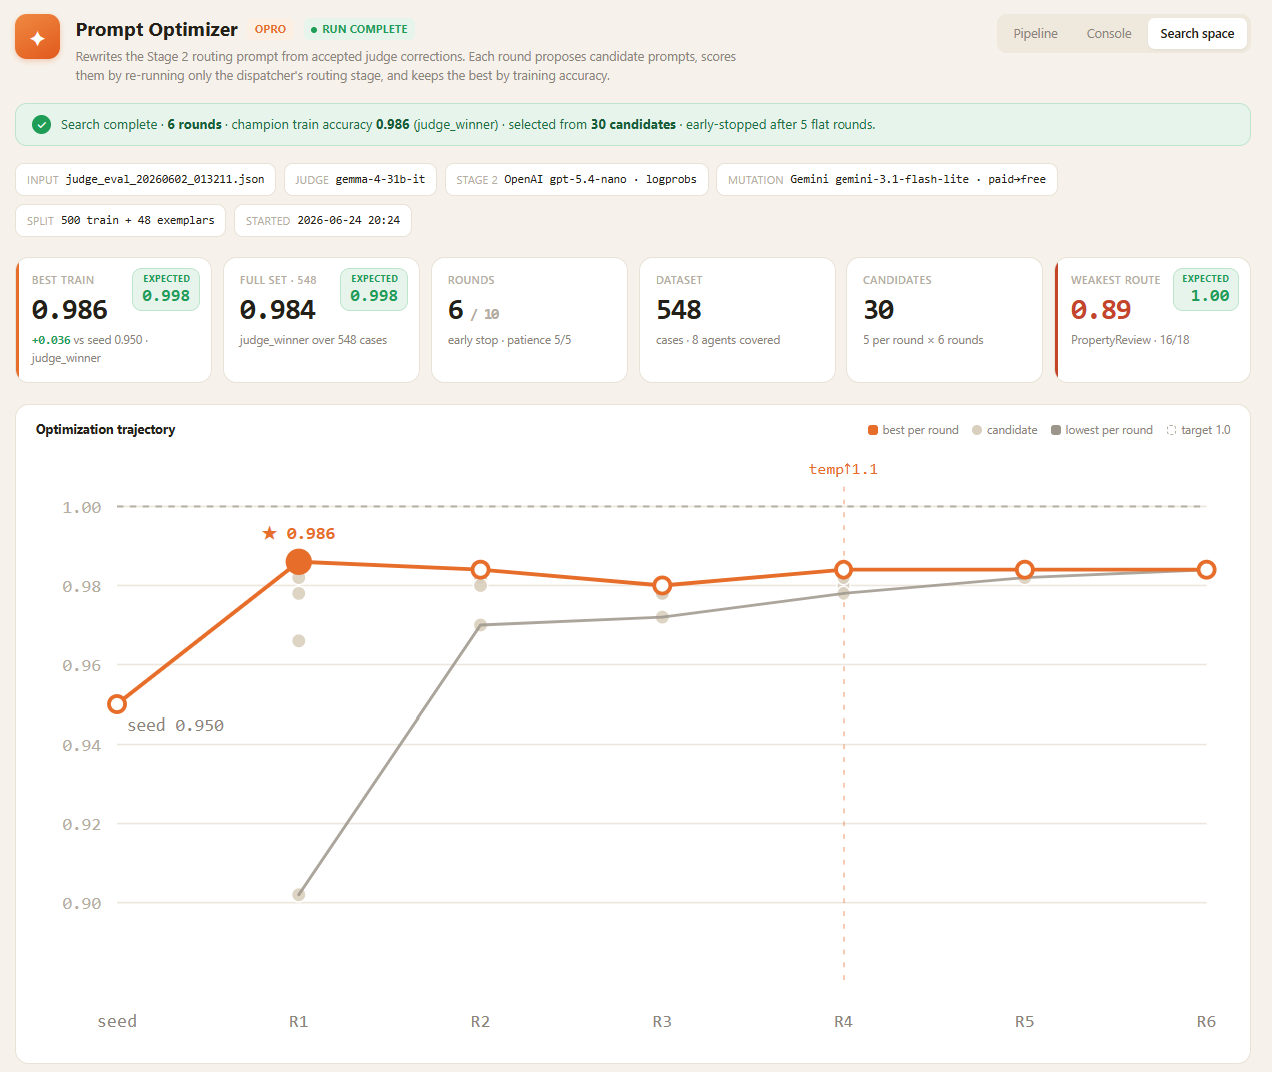
\includegraphics[width=1\linewidth,height=\textheight,keepaspectratio]{assets/pipeline/optimization-dashboard.png}
\caption{Optimization dashboard for the run of 24 June 2026 (development dashboard).}\label{fig:optimization-dashboard}
\end{figure}

\subsubsection{Evaluation}\label{sec:optimizer-evaluation}

The run in \cref{fig:optimization-dashboard} was chosen deliberately, as it is one of the weakest runs the optimizer produced, on the hardest data we have, a 548-case sample of the third-iteration golden dataset (\cref{sec:dataset-stages}).

The seed prompt was already written by us to be a good example of a well-written routing prompt, and it scored 0.950. The champion appeared in round 1 at 0.986 and was never beaten: rounds 2 to 6 returned 0.984, 0.980, 0.984, 0.984, and 0.984, and the run stopped early after five flat rounds. On the headline metric, therefore, five of six rounds bought nothing.

Reading only the best column misses what the run demonstrates. The floor rose while the ceiling stood still. In round 1 the five candidates spanned 0.902 to 0.986, a spread of more than eight points, and by round 6 all five scored 0.984 and the spread had closed entirely (\cref{fig:optimization-dashboard}). The mutator was not producing a better champion, but it had stopped producing bad prompts, which is the trajectory doing its work: shown every scored attempt in ascending order, the model learned what a competent routing prompt looks like even after it had stopped finding a superior one. This is the mechanism the natural-language gradient is supposed to supply, visible in a run where the headline metric shows nothing.

The run also exercises the plateau-escape rule. After rounds 2 and 3 passed without improvement, round 4 was mutated at a temperature of 1.1 instead of 0.8 and then reverted. It did not break the plateau, which is the honest outcome to report: the escape is one bounded attempt at divergence, not a guarantee, and patience still ended the run as designed.

The most interesting result is the divergence between the two labels. Measured against the judge, the champion routes 0.984 of the full set correctly. Measured against the golden dataset labels, it routes 0.998, a single misroute in 548 cases (\cref{tbl:optimizer-champion}).

\begin{longtable}[]{@{}
  >{\raggedright\arraybackslash}p{(\linewidth - 6\tabcolsep) * \real{0.3400}}
  >{\raggedright\arraybackslash}p{(\linewidth - 6\tabcolsep) * \real{0.2000}}
  >{\raggedright\arraybackslash}p{(\linewidth - 6\tabcolsep) * \real{0.2100}}
  >{\raggedright\arraybackslash}p{(\linewidth - 6\tabcolsep) * \real{0.1500}}@{}}
\caption{Champion accuracy by agent under both labelings. Case counts differ because the judge and the golden dataset assign some queries to different agents.}\label{tbl:optimizer-champion}\tabularnewline
\toprule\noalign{}
\begin{minipage}[b]{\linewidth}\raggedright
Agent
\end{minipage} & \begin{minipage}[b]{\linewidth}\raggedright
By judge label
\end{minipage} & \begin{minipage}[b]{\linewidth}\raggedright
By golden label
\end{minipage} & \begin{minipage}[b]{\linewidth}\raggedright
Cases
\end{minipage} \\
\midrule\noalign{}
\endfirsthead
\toprule\noalign{}
\begin{minipage}[b]{\linewidth}\raggedright
Agent
\end{minipage} & \begin{minipage}[b]{\linewidth}\raggedright
By judge label
\end{minipage} & \begin{minipage}[b]{\linewidth}\raggedright
By golden label
\end{minipage} & \begin{minipage}[b]{\linewidth}\raggedright
Cases
\end{minipage} \\
\midrule\noalign{}
\endhead
\bottomrule\noalign{}
\endlastfoot
CoachAgent & 1.00 & 1.00 & 11 / 12 \\
EmailAgent & 0.98 & 1.00 & 266 / 264 \\
ExposeAgent & 1.00 & 1.00 & 34 / 35 \\
GeneralPurposeAgent & 0.98 & 0.99 & 114 / 114 \\
MarketInfoAgent & 0.98 & 1.00 & 52 / 51 \\
OfferAgent & 1.00 & 1.00 & 39 / 41 \\
PlatformSupportAgent & 1.00 & 1.00 & 14 / 15 \\
PropertyReviewAgent & 0.89 & 1.00 & 18 / 16 \\
Full set & 0.984 & 0.998 & 548 \\
\end{longtable}

The optimizer therefore outperforms the examiner it was trained against, and the reason is structural rather than accidental. A judge's errors on individual cases are largely inconsistent, since the same query judged twice can fall either way, whereas the distinctions that actually separate two agents recur across many cases. A prompt is a single instruction of at most a few thousand characters, scored on hundreds of cases at once, so it has no capacity to encode a case-by-case correction: it can only capture what generalizes. Idiosyncratic judge noise is not learnable at that granularity and is left behind, while the systematic signal survives. The trajectory reinforces this, because a candidate that happened to fit a few noisy labels does not score consistently well across rounds and is not carried forward.

The weakest route under the judge's labeling is PropertyReviewAgent at 0.89, which is the same boundary the router struggles with (\cref{sec:router}) and the one the golden labeling shows as clean, another sign that the residual disagreement is the judge's rather than the prompt's.
